\documentclass[a4paper]{article}

\usepackage[T1]{fontenc}
\usepackage[utf8]{inputenc}
\usepackage[english]{babel}
\usepackage{csquotes}
\usepackage{listings}
\usepackage{multicol}
\lstset{language=c,frame=single,captionpos=b}
\usepackage{hyperref}
\usepackage{amsmath}
\usepackage[backend=biber, sorting=none,maxbibnames=40]{biblatex}
\renewbibmacro{in:}{}
\addbibresource{ref.bib}
\usepackage{graphicx}
\usepackage{placeins}
\usepackage[margin=2.5cm]{geometry}
\usepackage{subcaption}
\usepackage[affil-it]{authblk}
\usepackage{color}
\usepackage{amssymb,amsmath}
\usepackage{subfloat}
\usepackage{float}

\begin{document}
\title{JAVA Assignment: Rubik's Cube}
\author{Stefano Sandonà}
\affil{Vrije Universiteit Amsterdam, Holland}
\date{}
		
\maketitle

\section{The Rubik's Cube}
\label{sec:rubiks_cube}

A Rubik's Cube is a puzzle designed by Mr Rubik. In a Rubik's Cube, each of the faces is covered by colored stickers. In the initial setting, all the stickers of a face are of the same color and different colors are used for different faces. After performing some random twists, the aim of the game is to twist the cube until every side returns to be of a single color. 

\section{The Sequential Algorithm}
\label{sec:seq_algo}
The idea behind the sequential algorithm is simple. From a starting cube, we can twist it in each axis, row and direction (Figure \ref{fig:tw}). For each cube of size \textit{S}, doing a twist, there are \textit{6*(S-1)} new possible cubes. In Figure \ref{fig:tree}, the exolution of the search is represented as a tree. It's easy to understand from the figure that there is a rapid growth of the tree, in fact at the tree level \textit{i} there are \textit{(6*(S-1))\textsuperscript{i}} nodes (cubes).
The used state space search strategy, is the \textbf{deepening depth-first search (IDDFS)}. A depth-limited search is run repeatedly, increasing the depth limit with each iteration until it reaches d, the depth of the shallowest goal state. When the bound is increased, the solution search starts again from the begin (the root), and continues until the bound level is reached. On each iteration, the algorithm visits the nodes in the search tree in the same order as depth-first search, but the cumulative order in which nodes are first visited is effectively breadth-first. The first 2 iterations of the algorithm, with the order of the cube's evaluation is shown in Figure \ref{fig:iterations}.

\begin{figure}[ht]
  \centering
  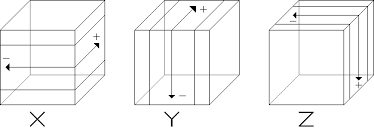
\includegraphics[width=0.5\linewidth]{xyz}
  \caption{Possible directions and axis for twists in a 3d cube}
  \label{fig:tw}
\end{figure}
\FloatBarrier

\begin{figure}[ht]
  \centering
  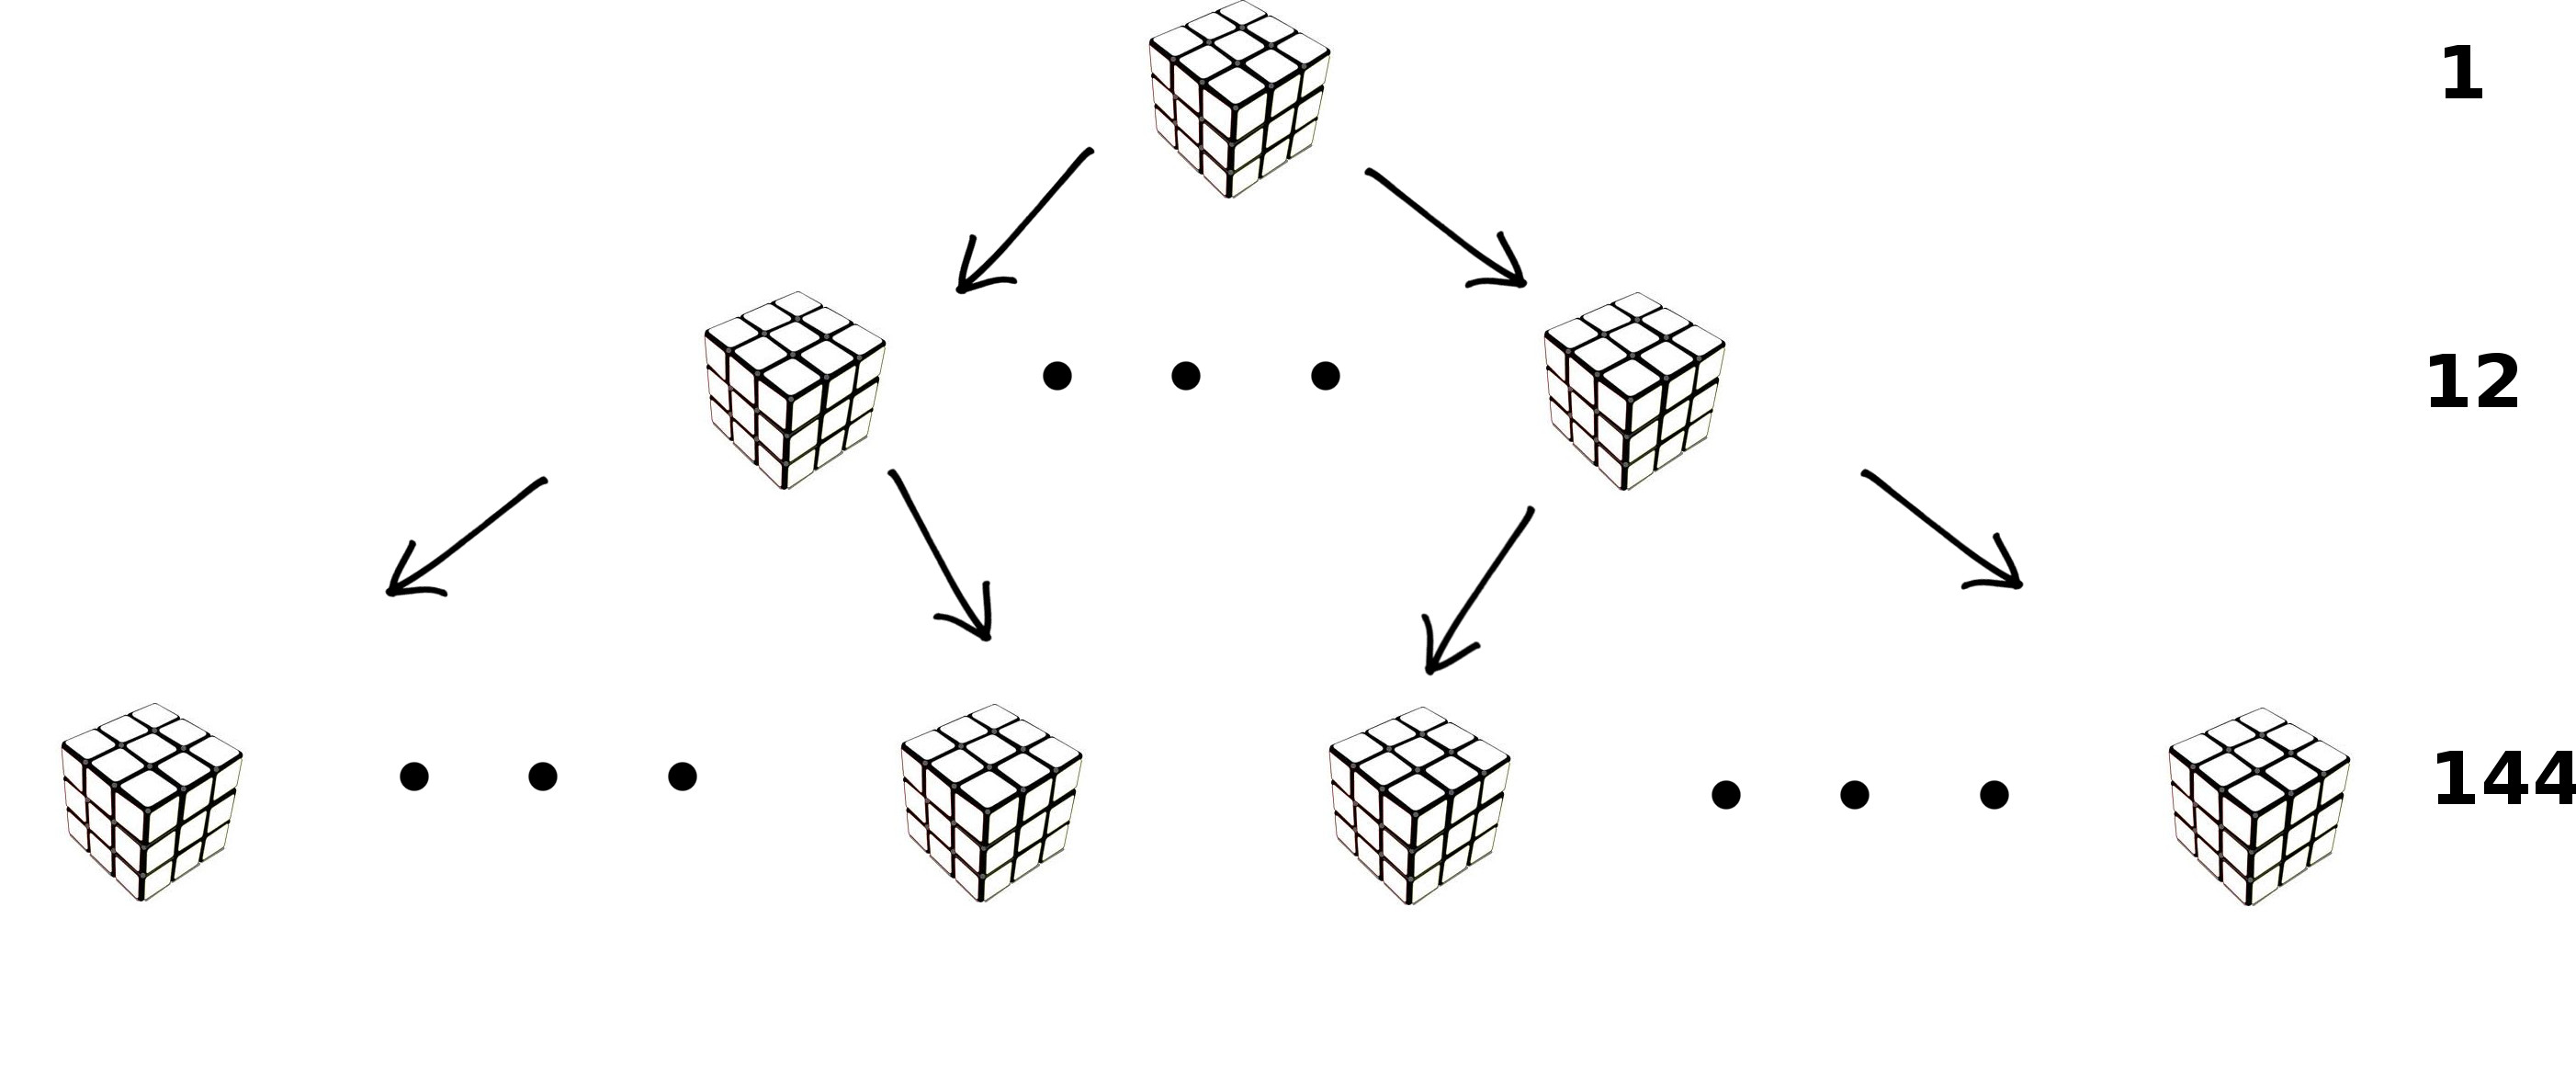
\includegraphics[width=0.8\linewidth]{rubik_tree}
  \caption{Rubik's Cube Solution Tree}
  \label{fig:tree}
\end{figure}
\FloatBarrier


\begin{figure}
\begin{subfigure}{0.40\textwidth}
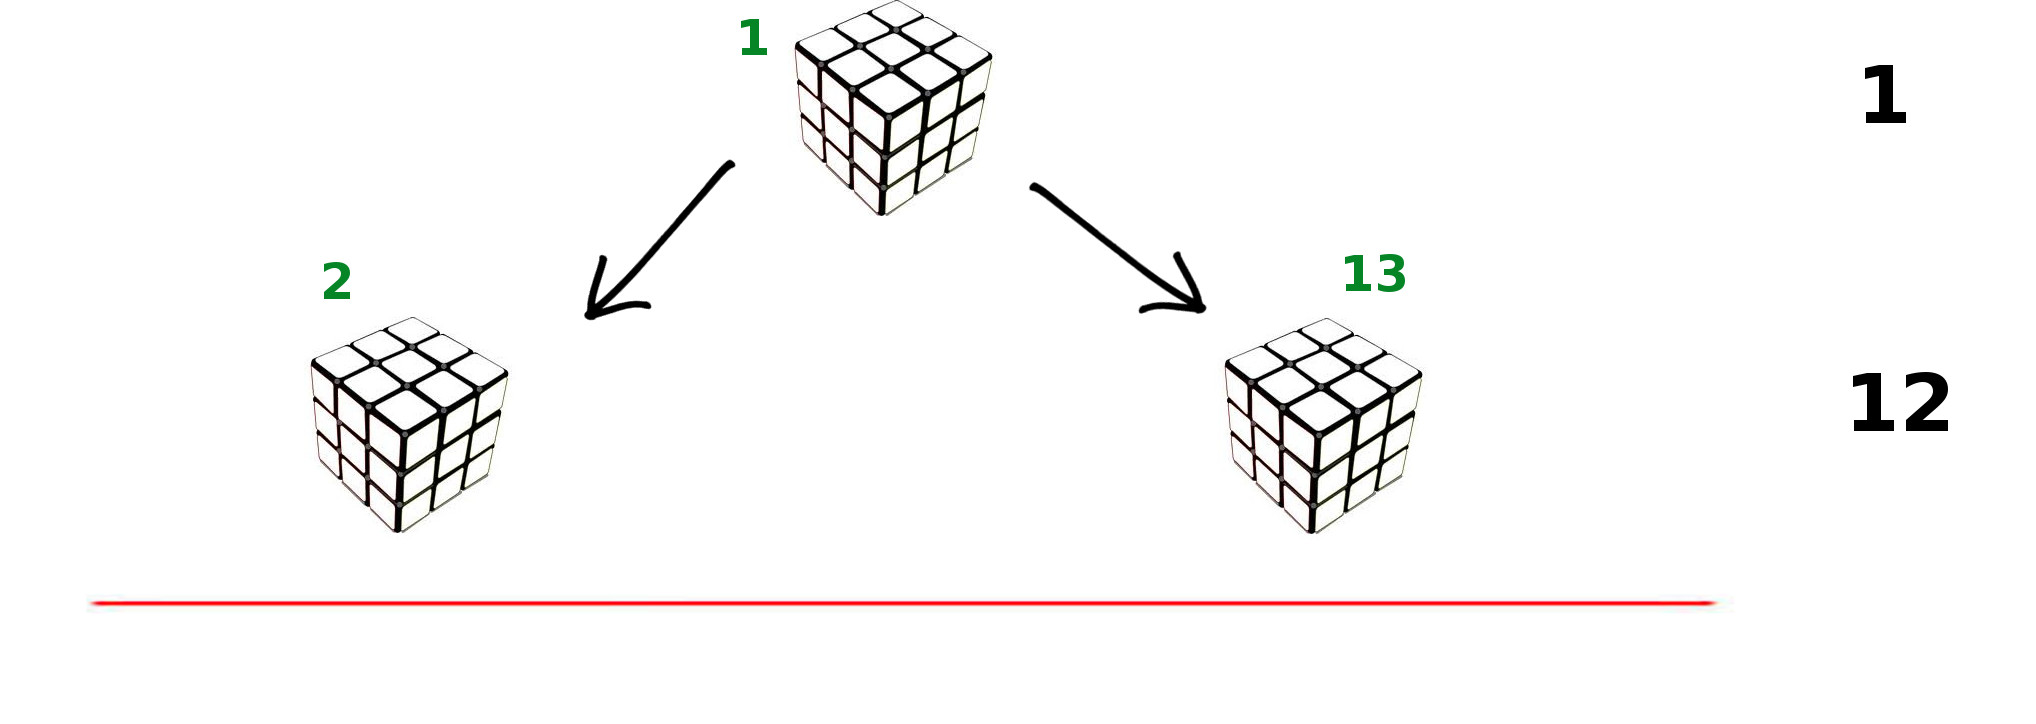
\includegraphics[width=\linewidth]{rubik_tree_eval1}
\caption{First itaration (bound=1)} \label{fig:ita}
\end{subfigure}
\hspace*{\fill} % separation between the subfigures
\begin{subfigure}{0.60\textwidth}
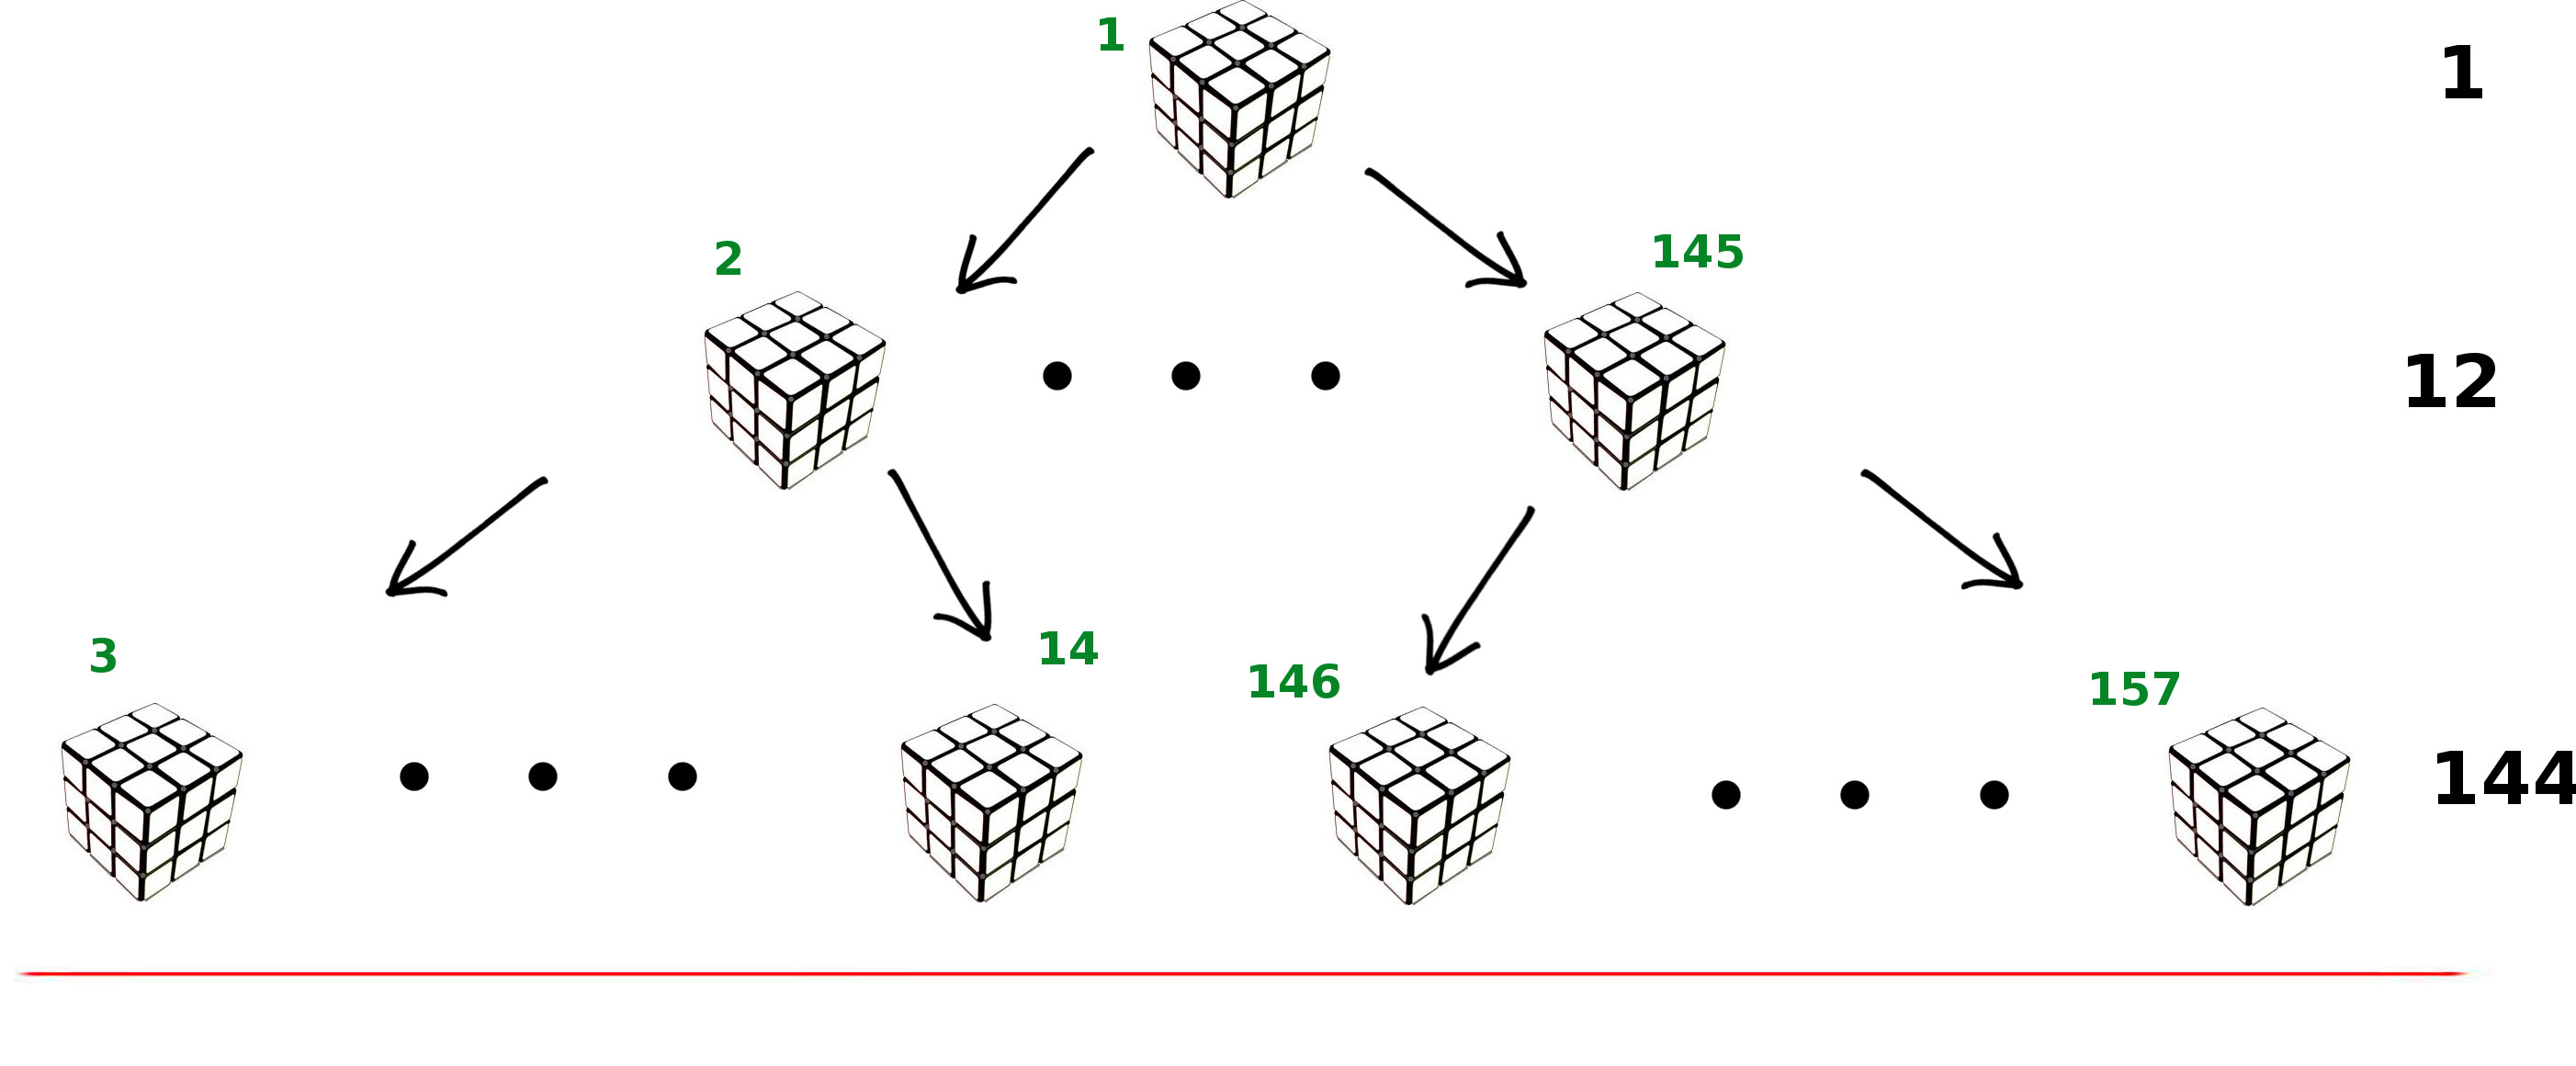
\includegraphics[width=\linewidth]{rubik_tree_eval2}
\caption{Second itaration (bound=2)} \label{fig:itb}
\end{subfigure}
\caption{The IDDFS Algorithm} \label{fig:iterations}
\end{figure}
\FloatBarrier

\section{The Parallel Algorithm}
\label{sec:par_algo}

\subsection{The Ibis Portability Layer (IPL)}
\label{sec:ibis}
The Ibis Portability layer (IPL) is a communication library specifically designed for usage in a grid environment. It is based on setting up connections. The programmer can create send/receive ports and connect them in a flexible way: one-to-one, one-to-many, many-to-one. In addition, the programmer can define properties of connections and ports like realiability, FIFO ordering, ... . This flexible message passing library for Java, is the core of the Ibis system, a Java-centric communication system designed for grid computing. A central concept in Ibis is the Pool. A pool consists of one or more Ibis instances,usually running on different machines. Each pool is generally made up of Ibises running single distributed application. Ibises in a pool can communicate with each other,
and, using the registry mechanism present in Ibis, can search for other Ibises in the
same pool, get notified of Ibises joining the pool, etc. To coordinate Ibis pools a socalled Ibis server is used.

For the parallel implementation of Rubik's Cube solver, this library was used.



An efficient parallelization of this algorithm is not trivial because of the work distribution. At each tree level there are \textit{(6*(S-1))\textsuperscript{i}} cubes, and this number is most likely not a multiple of the available nodes involved on the computation.
is easy to encounter load imbalance problems. The most balanced is the work among the involved nodes and the most is the performance.

\subsection{Cubes distribution}
\label{sec:cubes_distr}


\begin{equation} 
\label{eq:eq1}
\frac{(\sum_{i=0}^{m-z}{n^i}*\lfloor\frac{n^z}{k}\rfloor +  \sum_{i=0}^{m-z}{n^i})*100}{(\sum_{i=0}^{m-z}{n^i}*\lfloor\frac{n^z}{k}\rfloor)} < 101
\end{equation}

\begin{equation} 
\label{eq:eq1}
\lfloor\frac{n^z}{k}\rfloor > 100
\end{equation}

\begin{equation} 
\label{eq:eq1}
\sum_{i=0}^{m-z}{n^i}*\lfloor\frac{n^z}{k}\rfloor
\end{equation}

\begin{equation} 
\label{eq:eq1}
\sum_{i=0}^{m-z}{n^i}*\lfloor\frac{n^z}{k}\rfloor +  \sum_{i=0}^{m-z}{n^i}
\end{equation}

\printbibliography 

\end{document}